\chapter{3-D Convolutional Nerual Networks}
\label{4.3D_CNN}
\lhead{\emph{3-D Convolutional Neural Networks}}

Finally, with the release of PyEDDL version 1.0.0 less than a month ago, which supports 3-D CNN, we were able to test this approach to the MS lesion segmentation problem. The model implemented was introduced in 2017 in \cite{VALVERDE:2017} and consists on two 3-D CNN models in cascade. 

\section{Data preprocessing}

For this model we use \textit{FLAIR}, \textit{T1} and \textit{T2} modalities of the MRI images. First, the intensities of the images are normalized in order to speed up training and then for each of these we compute 3-D axial patches of size 11, centered on the voxel of interest and, obviously, keeping the correspondence voxel-mask label. The selection of the patch size is again the dilemma of losing context information or increasing data and model complexity and training and evaluation times. During preprocessing patches in which the voxel of interest has intensity lower than $0.5$ in the \textit{FLAIR} modality are removed.

Data agumentation is also performed by applying rotations to the patches, however, it's applied at batch time so it doesn't require any preprocessing. After the previous steps, the input is therefore a set of 3-D patches with three different channels corresponding the three modalities and size $(11\times11\times11)$.

Note that we implemented the data preprocessing manually, however, the second main component of the DeepHealth framework, the ECVL library, is intended to support common operations for biomedical images processing.


\section{Cascade model}

The idea of the cascade model is that the output of the first model if used to decide the input of the second one. This way the second model can process and debug those patches (actually their output via the first model) in which the first model is known to be less accurate. The first model is trained to be more sensitive to detect possible candidate lesion
voxels and the second model is trained to reduce the number of misclassified voxels coming from the
first one.

The structure of the cascade model is shown below, for all the details as well as the structure of the 3-CNN models themselves we refer to \cite{VALVERDE:2017}.

\vspace{0.6cm}
\begin{center}
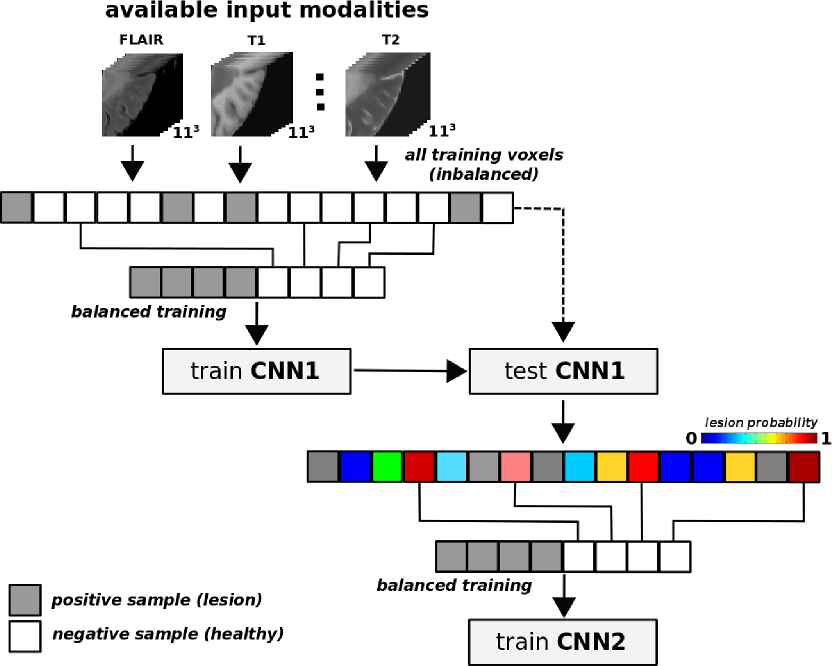
\includegraphics[width=\textwidth]{images/cascade_model.png}
\captionof{figure}{3-D Convolutional Neural Network cascade model \cite{VALVERDE:2017}}
\end{center}

%\newpage
%\subsection{Cascade model evaluation}

\newpage
\subsection{Cascade model CPU profiling}

The profiling was done under the same conditions as in \ref{U-Net CPU profiling}. We first analyze the training of both CNN models. The profiling shows a similar behaviour in both models, being the second one lighter in terms of memory usage. We can appreciate how the PyEDDL model is able to almost fully use all the CPUs available showing less insatiability than in previous more complex models.

Since both libraries achieve a similar CPU utilization, with less than a 10\% more for the TF models, the main differences are in the memory usage. Apparently, this goes against the conclusions obtained in all the previous profiles. In fact, at first it could look like an error in the measurements, however, this memory profile was repeated in several independent executions. 

After reviewing the code, we could see that the key behind this huge difference is the usage of \textit{generator functions}. These yield the data when it's required, while the \textit{fit} method in TF loads the whole data passed as parameter. Therefore we conclude that this difference is due to having non-equivalent implementations for both libraries and not due to the libraries themselves.


\begin{figure*}[!htb]
    \subfigure[Model 1 training CPU usage (\%) ]{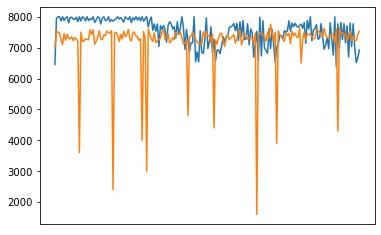
\includegraphics[width=.48\textwidth]{images/3d_model/profiles/model1_tr_cpu.jpg}}\hfill
    \subfigure[Model 2 training CPU usage (\%)]{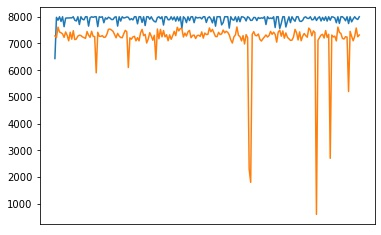
\includegraphics[width=.48\textwidth]{images/3d_model/profiles/model2_tr_cpu.jpg}}
    
    \subfigure[Model 1 training memory usage (GB)]{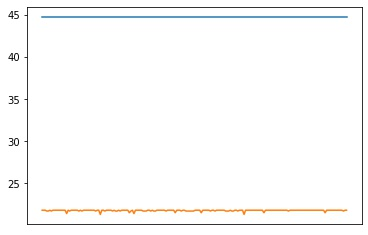
\includegraphics[width=.48\textwidth]{images/3d_model/profiles/model1_tr_mem.jpg}}\hfill
    \subfigure[Model 2 training memory usage (GB)]{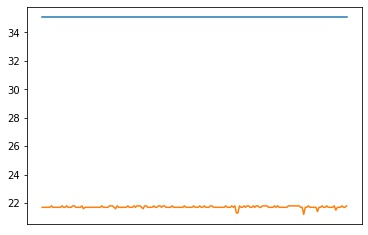
\includegraphics[width=.48\textwidth]{images/3d_model/profiles/model2_tr_mem.jpg}}
    \caption{Models training profile}
\end{figure*}

In the case of the models' evaluation we see a very significant  difference. Again the memory usage of the PyEDDL model is much lower but now, the ratio cpu-memory usage is much worse in this library than in TF. This is because, while the TF models are able to almost fully utilize all the CPUs, PyEDDL is using only one out of the 80 availables. We suppose this is because in PyEDDL 1.0.0 3-D CNN computations can not be parallelized since these have been just added to the library.

It's clear that this is a major drawback of this library. It increases severely the evaluation time, in our case up to seventy times more but we can't forget that it's a library currently in development, so it's more a drawback of the version.  

\begin{figure*}[!htb]   
    \subfigure[Model 1 evaluation CPU usage (\%) ]{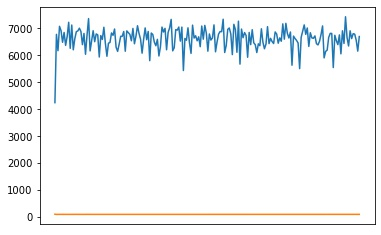
\includegraphics[width=.48\textwidth]{images/3d_model/profiles/model1_ts_cpu.jpg}}\hfill
    \subfigure[Model 2 evaluation CPU usage (\%) ]{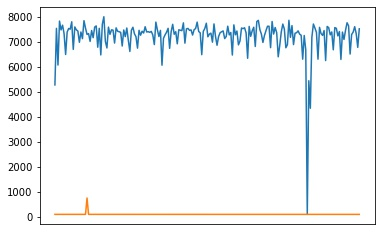
\includegraphics[width=.48\textwidth]{images/3d_model/profiles/model2_ts_cpu.jpg}}

    \subfigure[Model 1 evaluation memory usage (GB)]{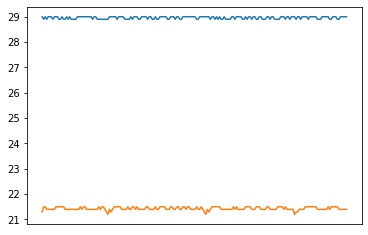
\includegraphics[width=.48\textwidth]{images/3d_model/profiles/model1_ts_mem.jpg}}\hfill
    \subfigure[Model 2 evaluation memory usage (GB)]{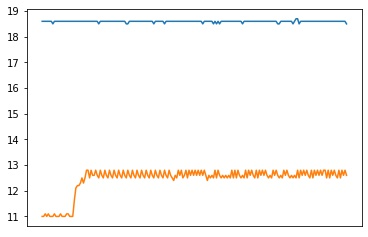
\includegraphics[width=.48\textwidth]{images/3d_model/profiles/model2_ts_mem.jpg}}
    \caption{Models evaluation profile}
\end{figure*}

Finally we have to add that we couldn't run this cascade model on GPU (and therefore we couldn't profile it) because due to an inner bug in the library, we were receiving a \textit{segmentation fault}.